\documentclass[9pt,pdf,utf8,hyperref={unicode},aspectratio=169]{beamer}

%Привычный шрифт для математических формул
\usefonttheme[onlymath]{serif}
\mode<presentation>
{
    \usetheme{boxes}
    \beamertemplatenavigationsymbolsempty

    \setbeamercovered{transparent}
    \setbeamertemplate{navigation symbols}{}
    
    \setbeamertemplate{footline}[frame number]
    \setbeamertemplate{caption}[numbered]
    % \setbeamersize{text margin left=0.5em, text margin right=0.5em}
}

% Дополнительные библиотеки
\usepackage[T2A]{fontenc}
\usepackage[english, russian]{babel}
\usepackage[utf8]{inputenc}
\usepackage{amsmath,amssymb}
\usepackage{indentfirst}
\usepackage{changepage}
\usepackage{enumerate}
\usepackage{mathtools}
\usepackage{multicol}
\usepackage{multirow}
\usepackage{ragged2e}
\usepackage{multicol}
\usepackage{diagbox}
\usepackage{wrapfig}
\usepackage{comment}
\usepackage{subfig}
\usepackage{array}
\usepackage{color}
\usepackage{tikz}
\usepackage{url}
\usepackage{bm}

\usetikzlibrary{trees}

% Определение дополнительных функций
\DeclareMathOperator*{\plim}{\mathop{plim}}
\DeclareMathOperator{\prob}{\mathbf{P}\!}

\DeclareMathOperator{\arctanh}{arctanh}
\DeclareMathOperator{\mmode}{mode}
\DeclareMathOperator{\rank}{rank}
\DeclareMathOperator{\diag}{diag}
\DeclareMathOperator{\sign}{sign}
\DeclareMathOperator{\cov}{cov}
\DeclareMathOperator{\pow}{pow}
\DeclareMathOperator{\med}{med}

\DeclareMathOperator*{\argmin}{arg\,min}
\DeclareMathOperator*{\argmax}{arg\,max}


\newcommand{\tsum}{\mathop{\textstyle\sum}\limits}
\newcommand{\condprob}[2] {\mathbf{P}\!\left(#1\left|#2\right.\right)}

\renewcommand{\leq}{\leqslant}
\renewcommand{\geq}{\geqslant}

\DeclareMathOperator{\FWER}{FWER}
\DeclareMathOperator{\FDR}{FDR}
\newtheorem{Th}{Теорема}
\newtheorem{Def}{Определение}

% Основная часть

\title[Введение в байесовскую статистику]{Прикладной статистический анализ данных\\Введение в байесовскую статистику}
\author{Андрей Грабовой}
\date{}

\begin{document}
\tikzstyle{every node}=[draw=black,thick,anchor=west]
\tikzstyle{selected}=[draw=red,fill=red!30]
\tikzstyle{optional}=[dashed,fill=gray!50]

\begin{frame}
    \titlepage
\end{frame}

\section{Мотивация}
\begin{frame}{Пример}
\only<1>{Монетку подбросили 5 раз, и все 5 раз выпал орел. Какова вероятность выпадения решки?}

\only<2>{Монетку подбросили 5 раз, и все 5 раз выпал орел. Какова вероятность выпадения решки?

 \bigskip Подход на основе ММП (``фреквентисткий''): посчитаем вероятность выпадения решки по выборке. 
 
 Ответ: 0.}

\only<3>{Монетку подбросили 5 раз, и все 5 раз выпал орел. Какова вероятность выпадения решки? 

\bigskip Подход на основе ММП (``фреквентисткий''): посчитаем вероятность выпадения решки по выборке. 

Ответ: 0.\\
\bigskip

\textbf{Проблема:} выборка слишком мала, чтобы делать такие поспешные выводы о выпадении решки. Кроме того, мы можем предположить что монетка должна давать более-менее равномерные результаты (это наши априорные предположения).}

\end{frame}
% 1. Задача
% 2. Наивный метод

\begin{frame}{Бета-распределение}
    \begin{itemize}
    \item соответствует \textit{априорным} ожиданиям о распределении Бернулли
  	%\item интерпретация: ``эффективное количество наблюдений $w=1, w=0$''
  	\item при $n \to \infty$ сходится к $\delta$-распределению в точке ОМП распределения Бернулли.
    \end{itemize}
    
    \begin{center}
    	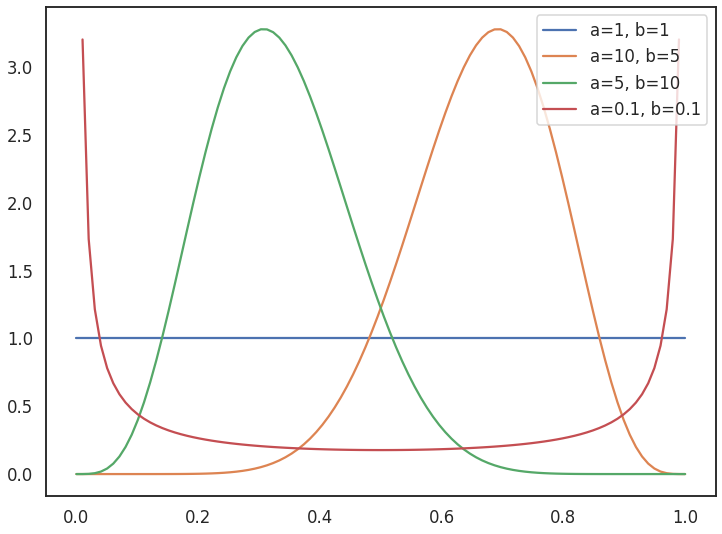
\includegraphics[width=0.5\textwidth]{beta.png}
    \end{center}
    
\end{frame}


\begin{frame}{Байесовский подход}
Введем бета-распределение в качетсве  \textcolor{red}{\textit{априорного}} предположения о распределении нашего параметра. Из общих соображений распределение должно быть симметрично (если у нас нет дополнительной информации):
\[
    \textcolor{red}{p(w)} \sim B(\alpha, \beta).
\]

Найдем \textit{апостериорное} распрделение параметра $w$ распределения Бернулли по формуле Байеса:
\[
    p(w|\boldsymbol{x}) = \frac{\textcolor{blue}{p(\boldsymbol{X}|w)} \textcolor{red}{p(w)}}{p(\boldsymbol{X})} \propto p(\boldsymbol{X}|w) p(w);
\]

$$\log p(w|\boldsymbol{x}) = \textcolor{blue}{\log p(\boldsymbol{X}|w)} + \textcolor{red}{\log p(w)} + \text{Const}.$$

\textbf{Вывод:} грубая интерпретация априорного распределения --- \textcolor{red}{регуляризатор}.

\end{frame}


\begin{frame}{Байесовский вывод: первый уровень}
Заданы:
\begin{itemize}
\item \textcolor{blue}{правдоподобие $p(\boldsymbol{X}|\boldsymbol{w})$} выборки $\boldsymbol{X}$ при условии параметра $\boldsymbol{w}$;
\item \textcolor{red}{априорное распределение $p(\boldsymbol{w}|\boldsymbol{h})$}
\item параметры априорного распределения $\boldsymbol{h}$ (В примере с монеткой: $\boldsymbol{h} = [\alpha, \beta];$)
\end{itemize}

Тогда апостериорное распределение параметров $\boldsymbol{w}$ при условии выборки $\boldsymbol{X}$:
$$p(\boldsymbol{w}|\boldsymbol{x}, \boldsymbol{h}) = \frac{\textcolor{blue}{p(\boldsymbol{X}|\boldsymbol{w})}\textcolor{red}{p(\boldsymbol{w}|\boldsymbol{h})}}{p(\boldsymbol{X}|\boldsymbol{h})} \propto p(\boldsymbol{X}|\boldsymbol{w}) p(\boldsymbol{w}|\boldsymbol{h}).$$

Точечная оценка параметров находится как максимум апостероирной вероятности (MAP):
\[
    \hat{\boldsymbol{w}} = \argmax \textcolor{blue}{p(\boldsymbol{X}|\boldsymbol{w})}\textcolor{red}{p(\boldsymbol{w}|\boldsymbol{h})}.
\]

MAP-оценка схожа с  оценкой методом максимального правдоподобия, если 
\begin{itemize}
\item Мощность выборка велика 
\item Априорное распределенеие --- равномерное на очень большой области 
\end{itemize}
\end{frame}




\section{Как работает байесовская статистика}
% Байес
% Формально
% Априорные - разные
% Гаус и лаплас
\begin{frame}{Байесовская статистика: пример}
Предположим, что параметр нашей модели (монетки) --- случайная величина.

Возьмем в качестве распределения модели --- бета-распределение с параметрами 2,2.

\begin{itemize}
\item $p(w) \sim \mathcal{B}(2,2)$ --- априорное распределение
\item $p(X|w)$ --- правдоподобие
\item $p(w|X) = \frac{p(w)p(X|w)}{p(X)}$ --- апостериорное распределение параметра.
\end{itemize}
\end{frame}



%https://www.thomasjpfan.com/2015/09/bayesian-coin-flips/
\begin{frame}
\only<1>{
\begin{figure}
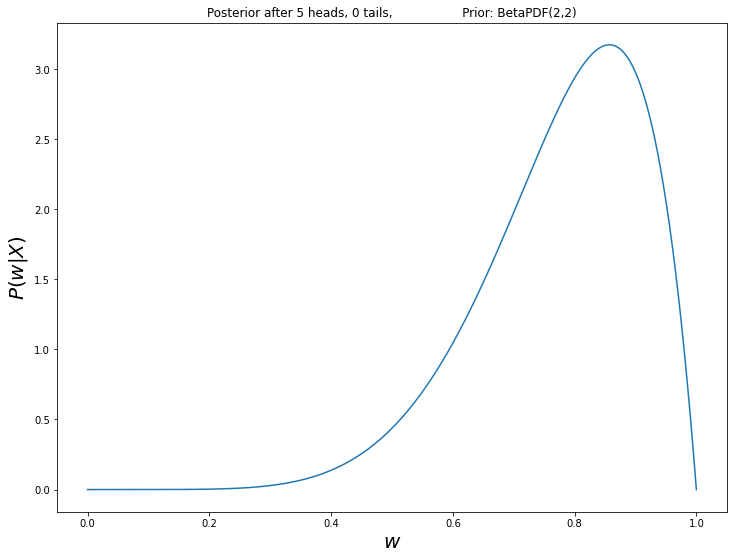
\includegraphics[width=0.75\textwidth]{coin1.png}
\end{figure}

В качестве ответа на вопрос из примера мы можем взять максимум апостериорной вероятности.
}

\only<2>{
\begin{figure}
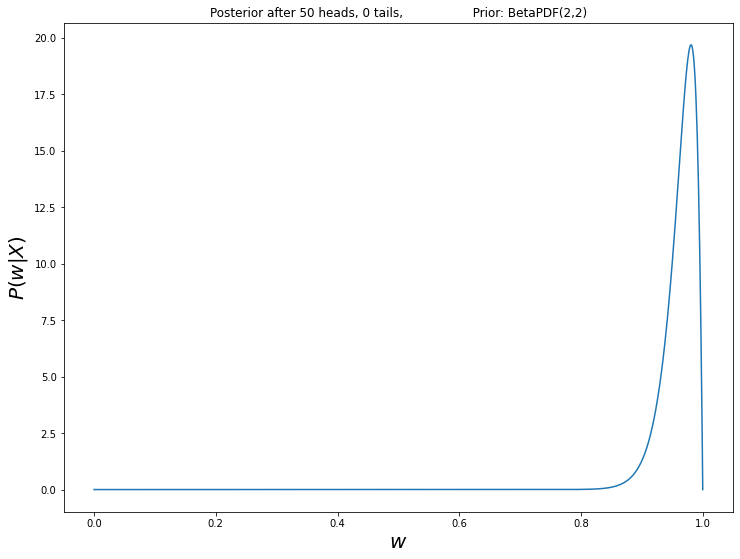
\includegraphics[width=0.75\textwidth]{coin2.png}
\end{figure}

}


\only<3>{
\begin{figure}
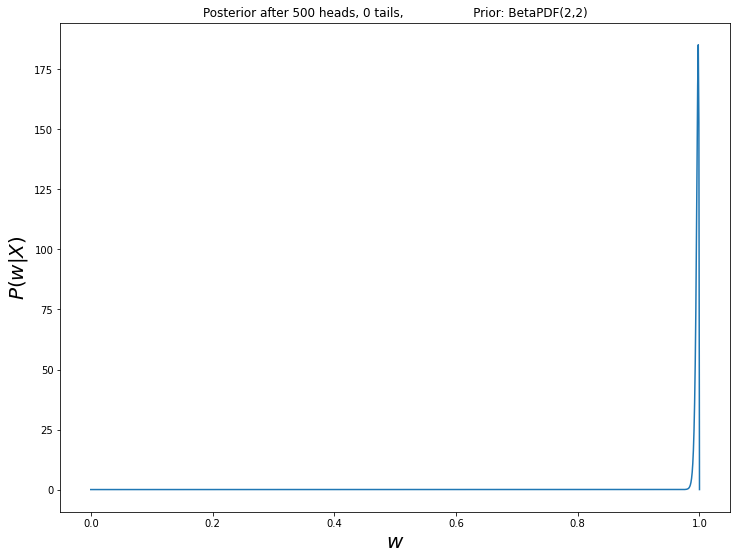
\includegraphics[width=0.75\textwidth]{coin3.png}
\end{figure}

}




\end{frame}


\begin{frame}{Почему для монетки подошло бета-распределение?}

$$p({w}|\boldsymbol{x}, \alpha, \beta) \propto \textcolor{blue}{p(\boldsymbol{X}|{w})}\textcolor{red}{p(w|\alpha, \beta)} \propto $$
$$ \propto w^{\sum {x}} (1-w)^{m - \sum{x}} \times  w^{\alpha-1}(1 - w)^{\beta - 1}  =$$
$$ = w^{\alpha-1 + \sum{x}}(1-w)^{m + \beta - \sum{x} - 1} \sim B(\alpha + \sum{x}, \beta + m - \sum{x}).$$

Семейство распределений называется сопряженным к распределению правдоподобия, если апостериорное распределение принадлежит этому же семейству.
\end{frame}


\begin{frame}{Формальная постановка}
\[
\hat{w} = \arg\max \frac{p(X|w)p(w)}{p(X)},
\]
\begin{itemize}
\item $p(w) \sim \mathcal{B}(2,2)$ --- априорное распределение, соответствующие нашим ожиданиям относительно параметра.
\item $p(X|w)$ --- правдоподобие.
\item $p(w|X) = \frac{p(w)p(X|w)}{p(X)}$ --- апостериорное распределение параметра.
\item $\hat{w}$ --- оценка, полученная методом максимума апостериорной вероятности (MAP).
\item $p(X)$ --- обоснованность модели (``Evidence'') --- насколько модель хорошо описывает выборку при разных значениях параметров.
\end{itemize}

\end{frame}


\begin{frame}{Как назначаются априорные распределения}
Априорные распределения назначаются на основе априорных ожиданий от поведения модели.

\textbf{Назначение априорного распределения, которое противоречит гипотезе о порождении данных --- некорректно}

Некоторые виды априорного распределения:
\begin{itemize}
\item Равномерное
\item Равномерное неограниченное
\item На основе предыдущих экспериментов
\item Для сдвигов
\begin{itemize}
\item Нормальное распределение
\item Распределение Лапласа
\end{itemize}
\item Для масштаба
\begin{itemize}
\item Гамма и обратное гамма-распределение
\item Коши (и производные)
\end{itemize}

\end{itemize}

\end{frame}

\begin{frame}{Распределение Джеффирса}
Распределение соответствует объему информации, хранимому в выбокре относительно параметров:
\[
	p(w) \propto \sqrt{\det I(w)}, 
\]
$I(w)$ --- информация Фишера:
\[
	I(w) \equiv  - \frac{\partial^2}{\partial w ^2}\log L\left(w\right).
\]
\begin{itemize}
\item Инвариантно относительно замены переменных;
\item Для среднего в нормальном распределении: $p(w) \propto 1$;
\item Для отклонения в нормальном распределении: $p(w) \propto \frac{1}{w}$;
\item Для параметра в распределении Бернулли: $p(w) \propto \frac{1}{\sqrt{p(1-p)}}.$
\end{itemize}
\end{frame}

\begin{frame}{Проблемы настройки параметров}
\only<1>{
	Если матрица $X$ вырождена, некоторые коэффициенты модели не будут определены. 
	
	\bigskip

	Если наблюдения $y=0$ и $y=1$ линейно разделимы в пространстве $X$, то:
	\begin{itemize}
	\item в теории коэффициенты бесконечно возрастают
	\item на практике коэффициенты и их дисперсии получаются большими, а~почти все вероятности в обучающей выборке близки к 0 или 1.
	\end{itemize}
	
	
	Можно использовать  регуляризацию Фирта. 
	Функция меток исходной модели для коэффициента $\beta_j$: $$\sum\limits_{i=1}^{n}\left(y_i - \pi\left(x_i\right)\right)x_{ij}.$$ 
	Регуляризованная версия: $$\sum\limits_{i=1}^{n}\left(y_i - \pi\left(x_i\right) + h_i\left(0.5-\pi\left(x_i\right)\right)\right)x_{ij},$$ 
	$h_i$~--- диагональный элемент hat matrix: $$H = V^{1/2}X\left(X^TVX\right)^{-1}X^TV^{1/2}.$$
}
\only<2>{
		\begin{center}
			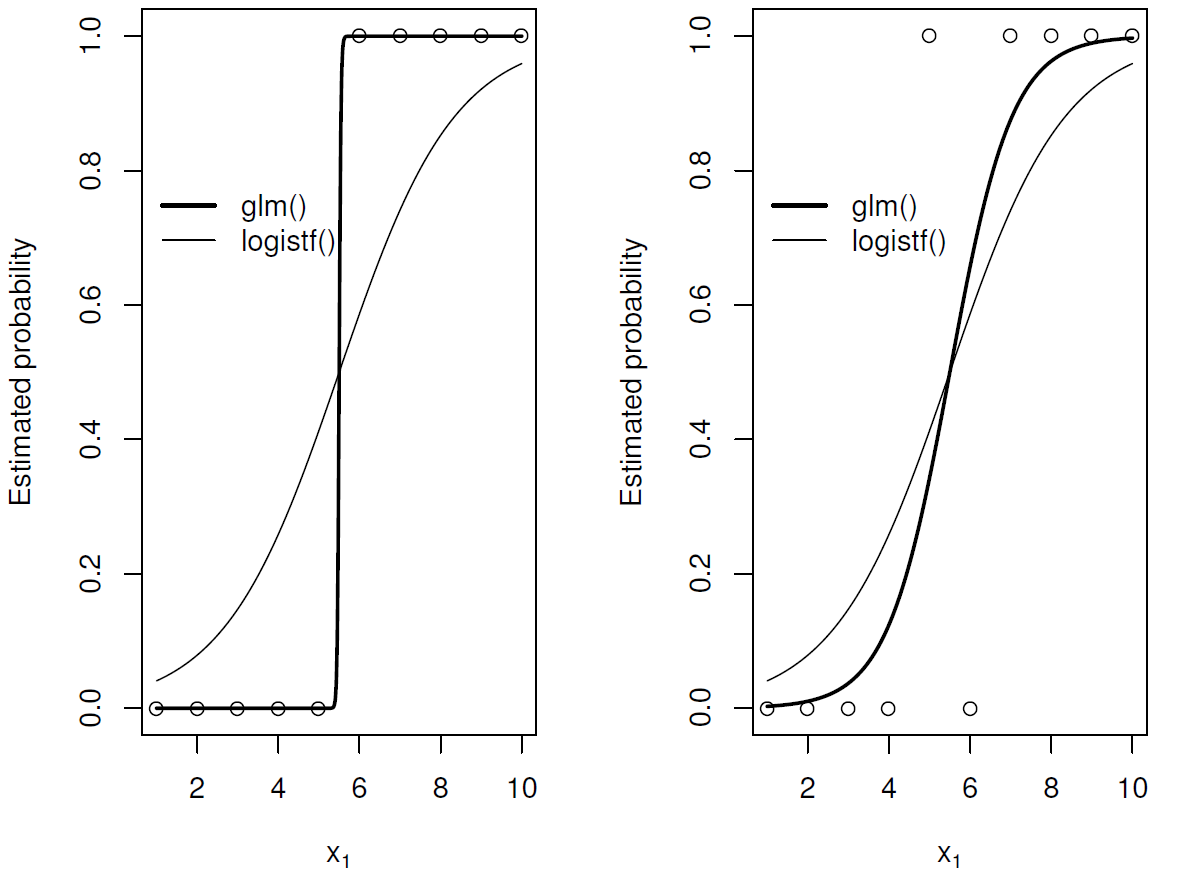
\includegraphics[width=0.65\textwidth]{separation.png}
		\end{center}	
	
}

\end{frame}


\begin{frame}{Нормальное распределение}
\[
	\log p(w|X) \propto \log p(w)p(X|w) \propto \log p(X|w) - \frac{(w-\mu)^2}{2\sigma^{2}}
\]
Получили $l_2$-регуляризацию.

При распределении Лапласа получаем $l_1$-регуляризацию.


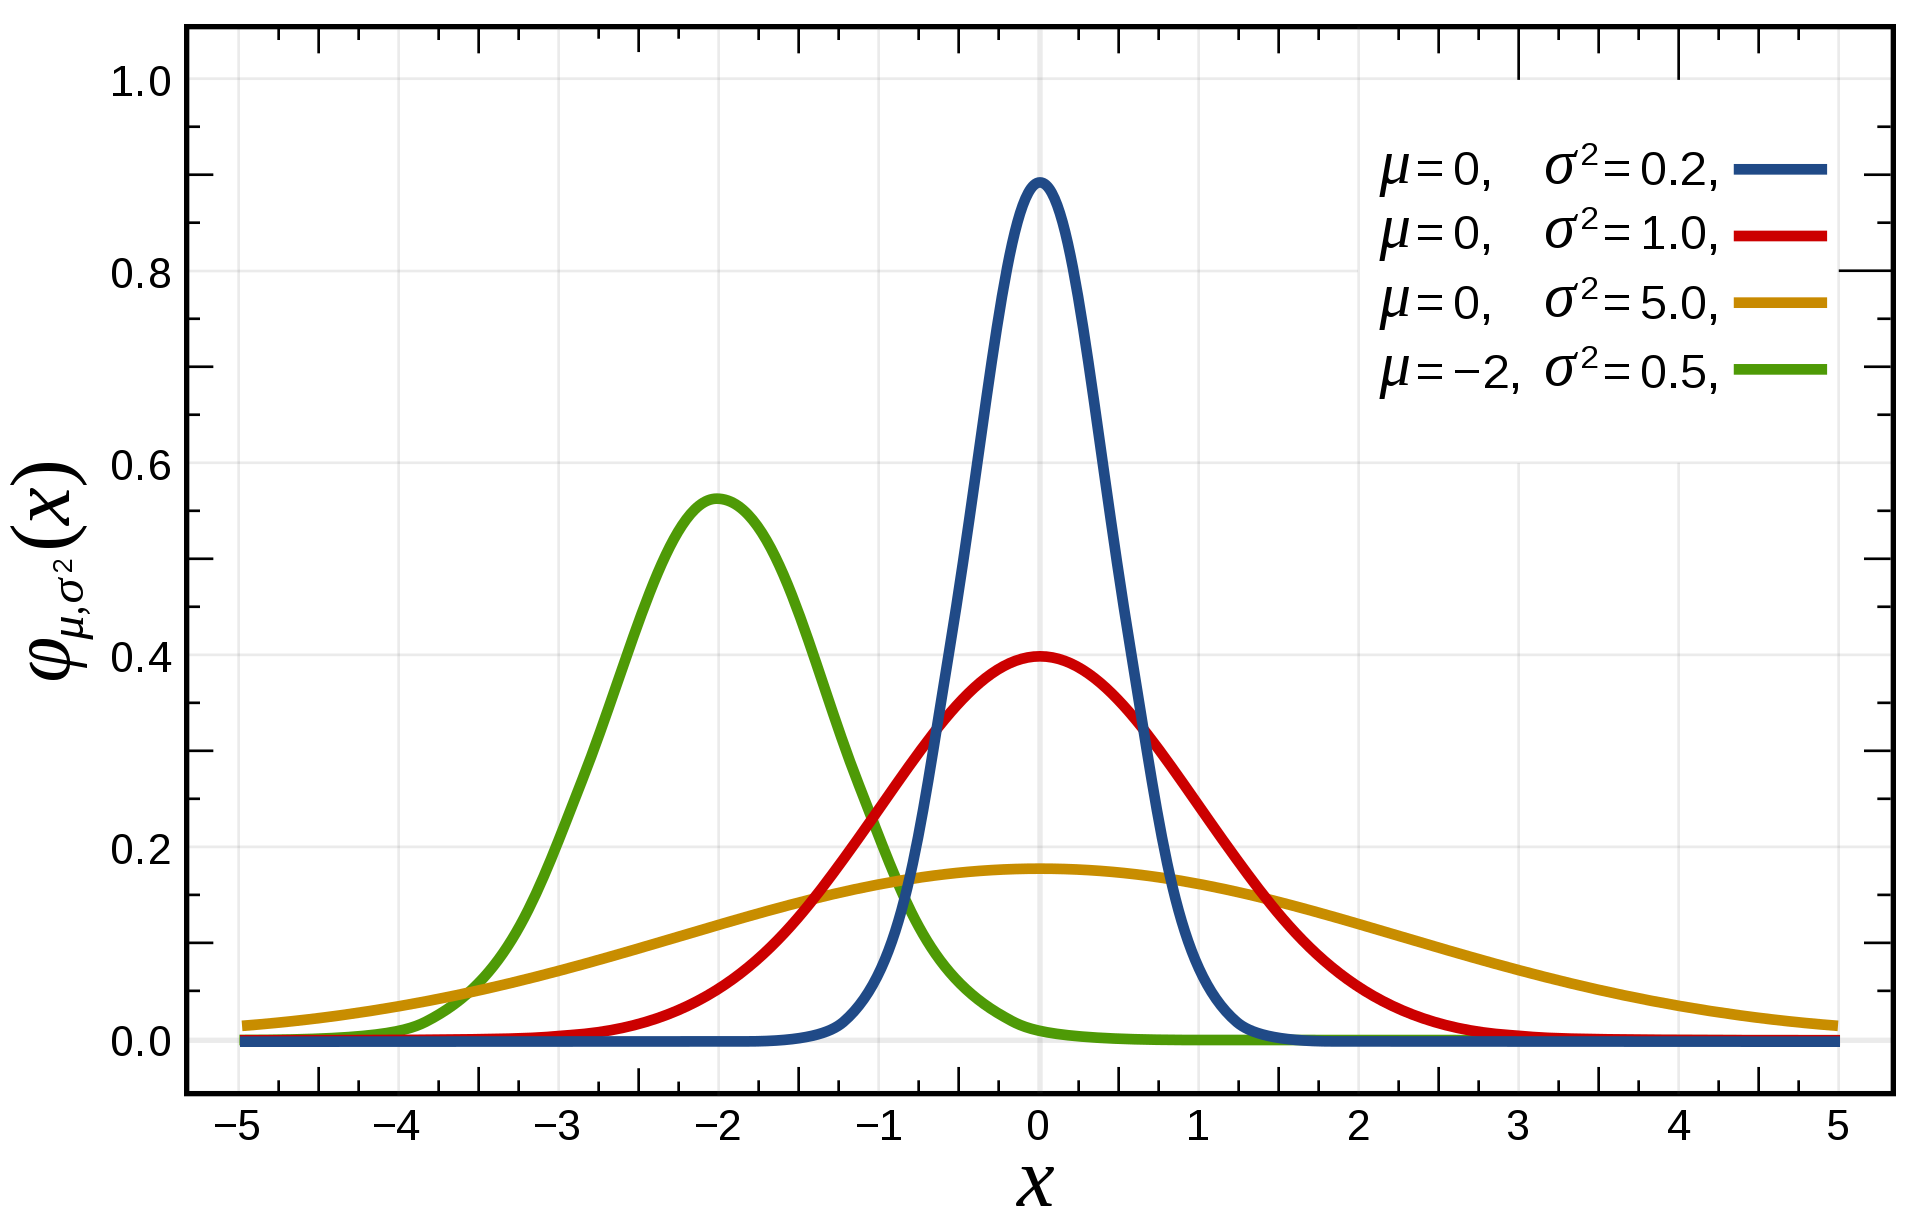
\includegraphics[width=0.4\textwidth]{gaus.png}
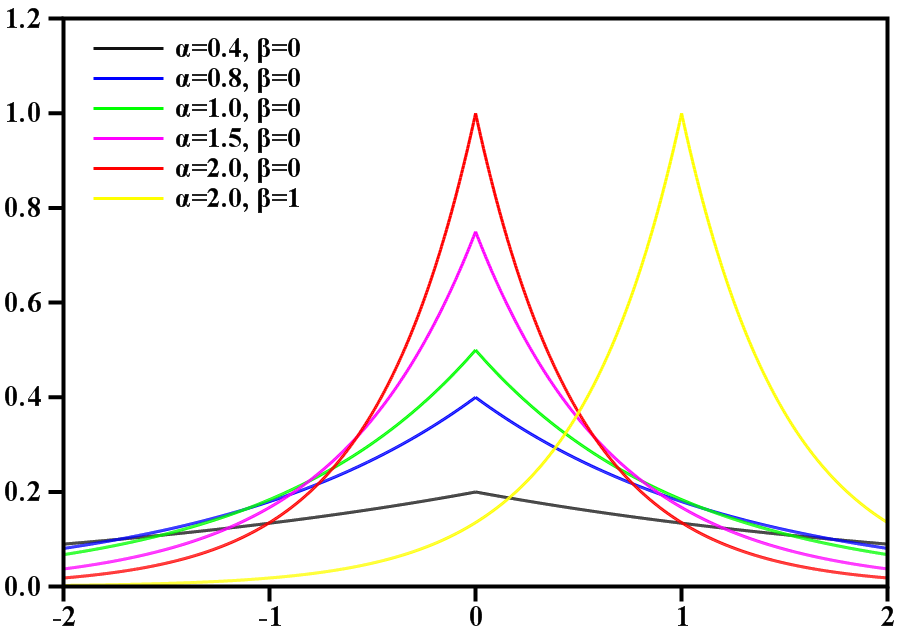
\includegraphics[width=0.37\textwidth]{laplace.png}


\end{frame}




\begin{frame}{Informative prior vs Uninformative prior}
\begin{itemize}
\item Informative prior: соответствует экспертным знаниям о наблюдаемой переменной 
\begin{itemize}
\item Пример: температура воздуха: нормальная величина с известным средним и дисперсией, соответствующими прошлым наблюдениям.
\end{itemize}

\item Uninformative prior: соответствует базовым предположениям о распределении переменной
\begin{itemize}
\item Пример: температура воздуха: равномерное распределение (improper).
\end{itemize}

\item Weakly-informative prior: где-то по середине
\begin{itemize}
\item Пример: температура воздуха: равномерное распределение от -50 до +50.
\end{itemize}


\end{itemize}


\end{frame}

% Как выбирать априорное распределение
\section{Доверительные интервалы}
\begin{frame}{Напоминание: Интервальные оценки}
%%%%%%%%%%%%%%%%%%%%%%%%%%%%%%%%%%%%%%%%%%%%%%%%%%%%%%%%%%%%%%%%%%%%%%%
% 
%%%%%%%%%%%%%%%%%%%%%%%%%%%%%%%%%%%%%%%%%%%%%%%%%%%%%%%%%%%%%%%%%%%%%%%
    Доверительный интервал:
    $$\prob\left(\theta \in \left[C_L, C_U\right]\right)\geq 1-\alpha,$$
    $1-\alpha$~--- уровень доверия, 
    
    $C_L$, $C_U$~--- нижний и верхний доверительные пределы.

    \bigskip

	\textbf{Неверная интерпретация}: неизвестный параметр лежит в пределах построенного доверительного интервала с вероятностью $1-\alpha$.
	
	\bigskip

	\textbf{Верная интерпретация:} при бесконечном повторении процедуры построения доверительного интервала на аналогичных выборках в~$100(1-\alpha)$\% случаев он будет содержать истинное значение $\theta$.
\end{frame}

\begin{frame}{Напоминание: для нормального распределения}
%%%%%%%%%%%%%%%%%%%%%%%%%%%%%%%%%%%%%%%%%%%%%%%%%%%%%%%%%%%%%%%%%%%%%%%
% по сути это более точная версия правил 2-3 сигм, обобщённая на произвольное количество сигм
%%%%%%%%%%%%%%%%%%%%%%%%%%%%%%%%%%%%%%%%%%%%%%%%%%%%%%%%%%%%%%%%%%%%%%%
	$X\sim N\left(\mu,\sigma^2\right),\;\; X^n=\left(X_1,\dots,X_n\right),$
	
	\bigskip
	
	$\bar{X}_n$~--- оценка $\mathbb{E}X=\mu,$
	\bigskip
	
    $\bar{X}_n\sim N\left(\mu, \frac{\sigma^2}{n}\right) \Rightarrow $
	$$\prob \left(\mu-z_{1-\frac{\alpha}{2}} \frac{\sigma}{\sqrt{n}}  \leq \bar{X}_n \leq \mu +z_{1-\frac{\alpha}{2}} \frac{\sigma}{\sqrt{n}} \right)=1-\alpha \Rightarrow $$
	
	доверительный интервал для $\mu$:
	$$\prob \left(\bar{X}_n-z_{1-\frac{\alpha}{2}} \frac{\sigma}{\sqrt{n}}  \leq \mu \leq \bar{X}_n +z_{1-\frac{\alpha}{2}} \frac{\sigma}{\sqrt{n}} \right)=1-\alpha,$$
	$z_{1-\frac{\alpha}{2}}$~--- квантиль стандартного нормального распределения.
\end{frame}


\begin{frame}{Байесовская интервальные оценка (credible interval)}
%%%%%%%%%%%%%%%%%%%%%%%%%%%%%%%%%%%%%%%%%%%%%%%%%%%%%%%%%%%%%%%%%%%%%%%
% 
%%%%%%%%%%%%%%%%%%%%%%%%%%%%%%%%%%%%%%%%%%%%%%%%%%%%%%%%%%%%%%%%%%%%%%%
    Доверительный интервал:
    $$\int_{w \in [C_L, C_U]}p(w|X) \geq 1-\alpha,$$
    $1-\alpha$~--- уровень доверия, 
    
    $C_L$, $C_U$~--- нижний и верхний доверительные пределы.

    \bigskip

	\textbf{Интерпретация:}  неизвестный параметр, породивший выборку, лежит в пределах построенного доверительного интервала с вероятностью $1-\alpha$.
	
\begin{itemize}
	\item Доверительные интервалы совпадают для параметров сдвига с равномерным распределением и масштаба с распределением Джеффриса.
\end{itemize}
\end{frame}

\begin{frame}{Пример}
\[
	X \sim \mathcal{N}(0,1), |X| = 10, \bar{X} = 0.17.
\]
\begin{itemize}
\item Доверительный интервал: [-0.45,0.78]
\item Prior: $\mu \sim \mathcal{N}(0, 0.01),$ доверительный интервал: [-0.002, 0.03].
\end{itemize}

\[
	X \sim \mathcal{N}(0,1), |X| = 100000, \bar{X} = 0.17.
\]
\begin{itemize}
\item Доверительный интервал: [0.1638,0.1763]
\item Prior: $\mu \sim \mathcal{N}(0, 0.01),$ доверительный интервал: [0.16981, 0.16984].
\end{itemize}



\end{frame}



\section{Выбор моделей}
\begin{frame}{Выбор моделей}
\textbf{Задан набор моделей, требуется определить, какой из них лучше подходит для работы с выборкой.}\\
\begin{itemize}
\item Линейная модель --- $R^2$ и пр.
\item Обобщенно-линейная модель --- остаточная аномальность.
\item Что делать, если модель нелинейная?
\item Что делать с параметрами априорного распределения, как их выбирать?
\end{itemize}

\end{frame}



\begin{frame}{AIC}
\[
	AIC = -2L + 2 (k+1),
\]
где $k$ --- количество параметров.

Критерий соответствует потерю в информации относительно истинного распределения данных:
\[
	AIC \approx KL(f|f_i), 
\]
где $f$ --- истинное распределение, $f_i$ --- модель-кандидат, описывающий распределение.
\end{frame}

\begin{frame}{Связанный байесовский вывод}
\textit{Первый уровень:} выбираем оптимальные параметры:
\[
    {w} = \arg\max \frac{p({X}|{w})p({w})}{p(X)},
\]

\textit{Второй уровень:} выбираем модель, доставляющую максимум обоснованности модели.

Обоснованность модели (``Evidence''):
\[
	p(X) = \int_w {p(X|w)}{p(w)} dw.
\]


\begin{figure}
  \centering
  \subfloat[Схема выбора модели]{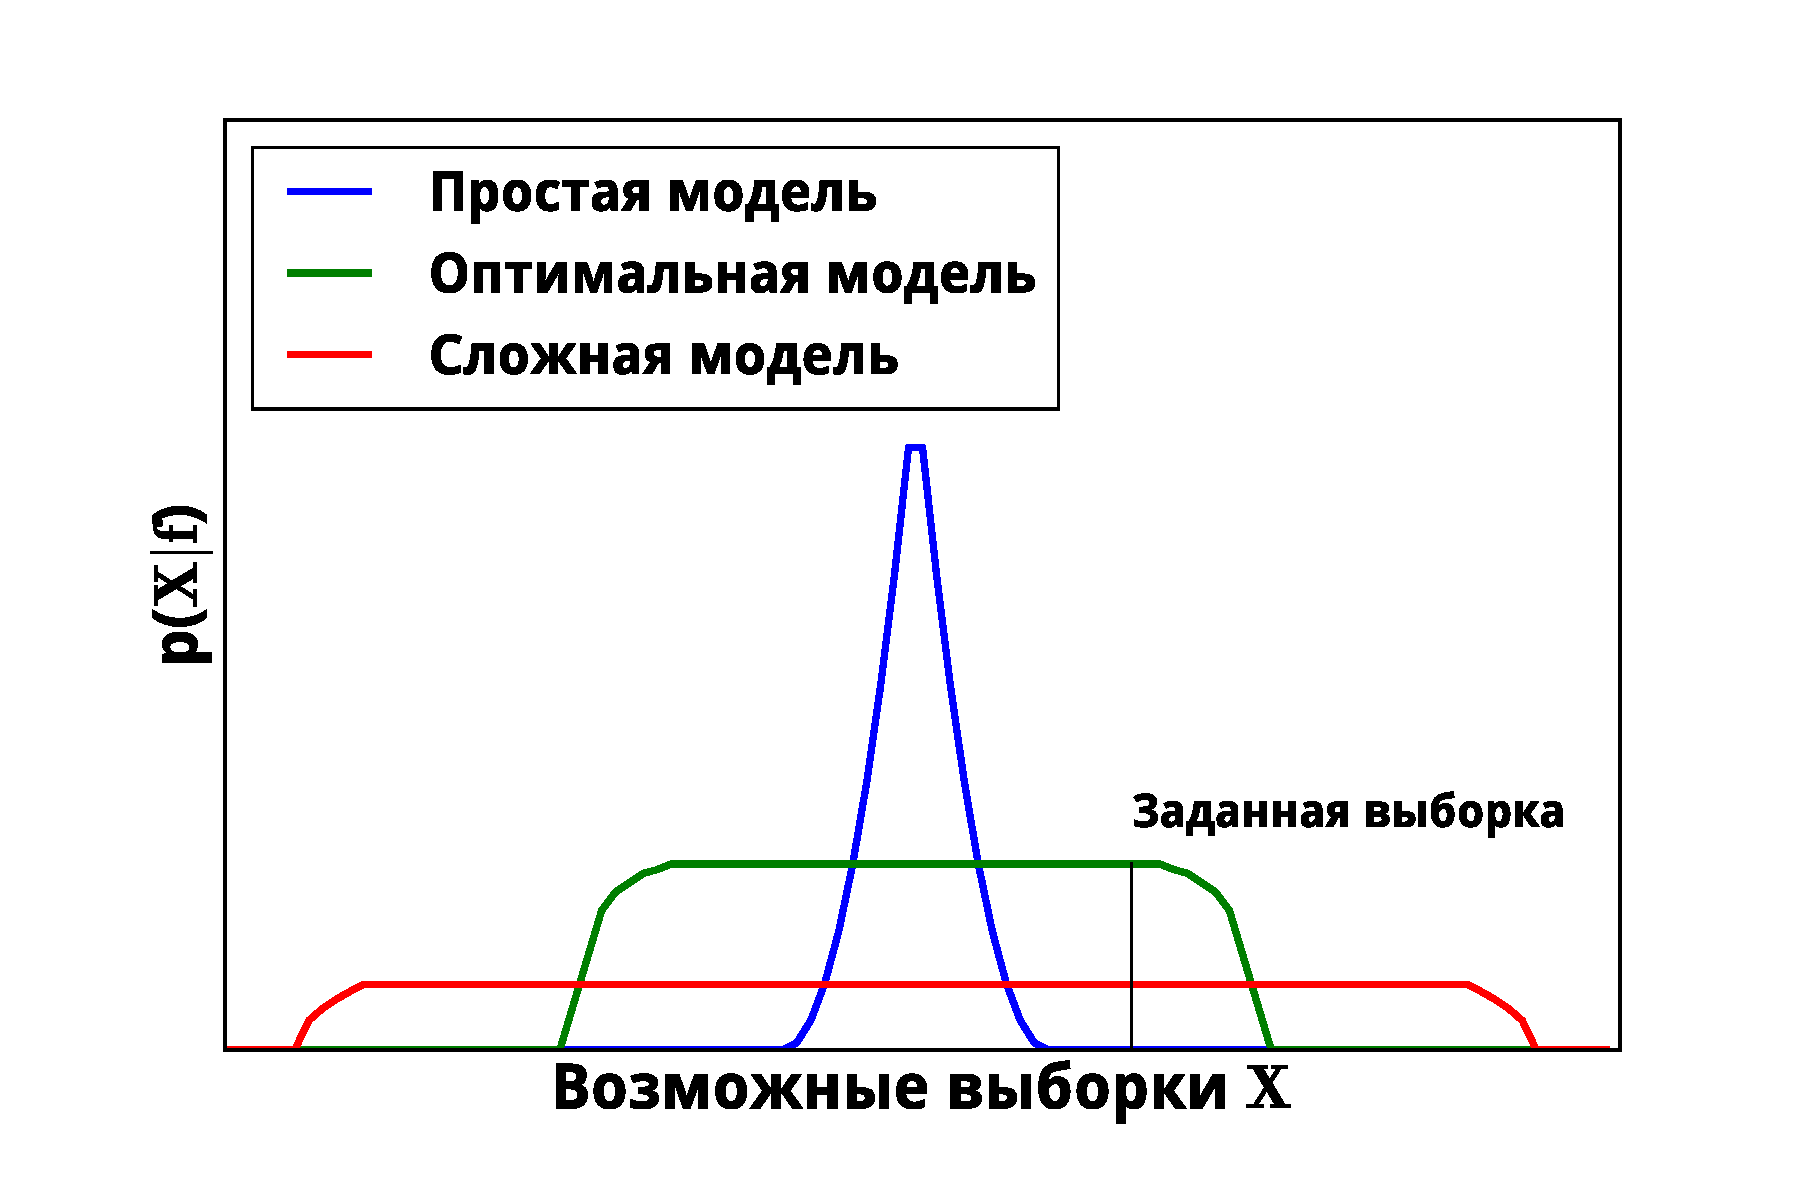
\includegraphics[width=0.4\textwidth]{evidence.pdf}} 
 \subfloat[Пример: полиномы]{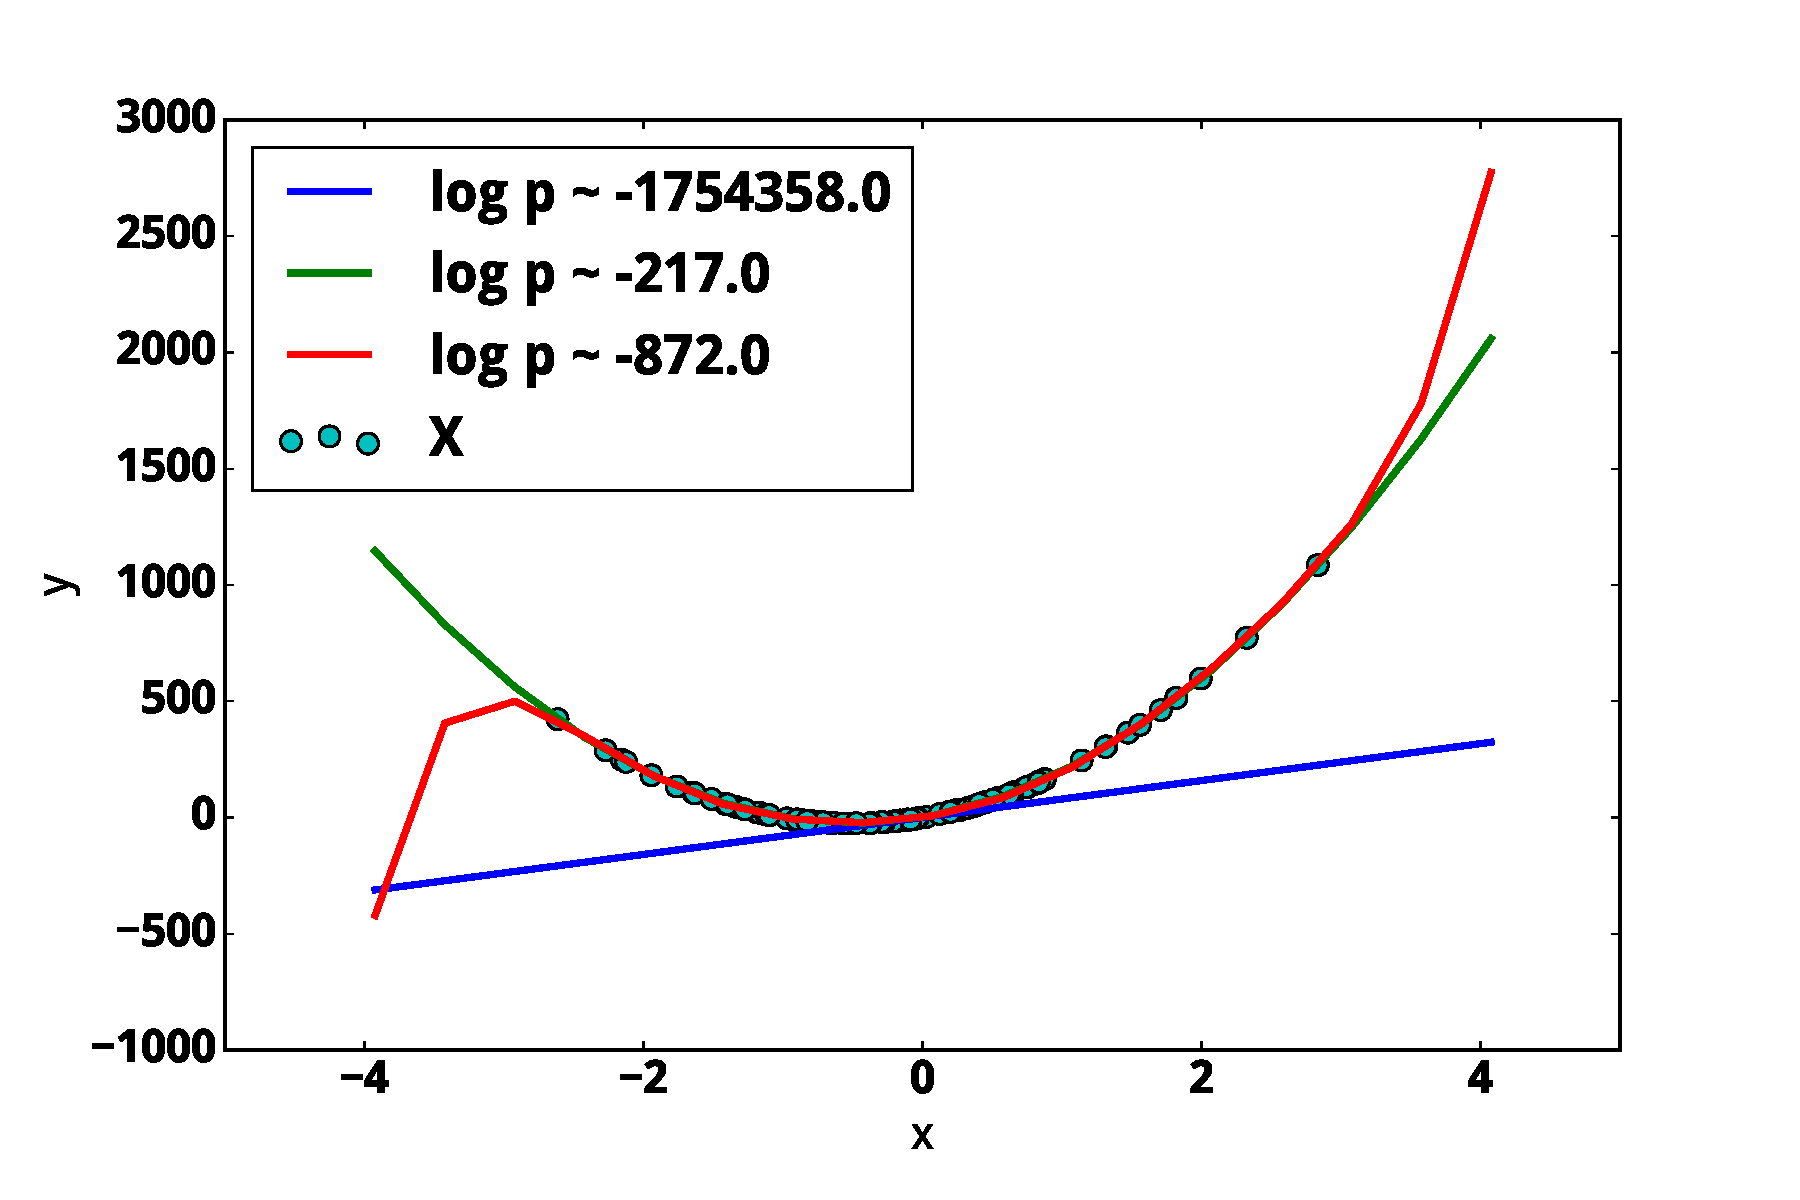
\includegraphics[width=0.4\textwidth]{example.pdf}}
\label{fig:1}\qquad

\end{figure}

\end{frame}



\begin{frame}{Принцип минимальной длины описания}
\[
\text{MDL}(\mathbf{f}, \mathfrak{D}) = L(\mathbf{f}) + L(\mathfrak{D}|\mathbf{f}),
\]
где $\mathbf{f}$ --- модель, $\mathfrak{D}$ --- выборка, $L$ --- длина описания в битах.

Аппркосимация этой величины для достаточно большой мощности выборки $n$:
\[
	BIC = -2L + \log n (k+1).
\]
\\
\[
\text{MDL}(\mathbf{f}, \mathfrak{D}) \sim L(\mathbf{f}) + \textcolor{blue}{L(\mathbf{w}^*| \mathbf{f})} + \textcolor{red}{L(\mathfrak{D}|\mathbf{w}^*, \mathbf{f})},
\]
$\mathbf{w}^*$ --- оптимальные параметры модели.\\

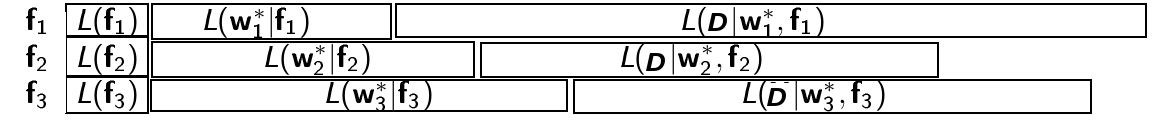
\includegraphics[width=\textwidth]{./mdl.png}

\end{frame}

\begin{frame}{MDL и Колмогоровская сложность}
\textbf{Колмогоровская сложность} --- длина минимального кода для выборки на предварительно заданном языке.

\textbf{Теорема инвариантности}\\
Для двух сводимых по Тьюрингу языков колмогоровская сложность  отличается не более чем на константу, не зависяющую от мощности выборки.\\

\textbf{Отличия от MDL}:
\begin{itemize}
\item Колмогоровская сложность невычислима.
\item Длина кода может зависеть от выбранного языка. Для небольших выборок теорема инвариантности не дает адекватных результатов.
\end{itemize}
\end{frame}
\begin{frame}{Evidence vs MDL}
\centering
\begin{tabular}{ c | c  }
  \hline			
 \bf Evidence & \bf MDL \\
  \hline  
Использует априорные знания &  Независима от априорных знаний \\
  \hline  
Основывается на гипотезе о порождении\\ выборки & Минимизирует длину описания выборки\\ вне зависимости от их природы \\
  \hline  

\end{tabular}
\end{frame}


\begin{frame}{Как считать Evidence?}
\begin{itemize}
\item Для линейных моделей: аналитическая формула
\item Для нелинейных моделей аппроксимация Лапласа:
\[
	p(X) = \int_w p(X, w)dw
\]
\begin{itemize}
\item Разложим $\log p(X|w)$ в ряд Тейлора:
\[
	\log p(X|w) \approx  \log p(X,w_0) - \frac{\partial^2}{2\partial w^2} \log p(X,w_0) (w-w_0)^2. 
\]

\item Вычислим интеграл для ненормированной гауссовой величины $p(x,w_0)\text{exp}(  - \frac{\partial^2}{2\partial w^2} \log p(X,w_0) (w-w_0)^2).$

\end{itemize}

\item MCMC, вариационный вывод и пр.


\end{itemize}
\end{frame}



\begin{frame}{Пример: линейная регрессия}
\small
Линейный случай с $m$ объектами и $n$ признаками:
$\boldsymbol{f}(\boldsymbol{X}, \boldsymbol{w}) = \boldsymbol{X}\boldsymbol{w};$
$\boldsymbol{y} \sim \mathcal{N}(\boldsymbol{f}(\boldsymbol{X}, \boldsymbol{w}), \beta^{-1}), \boldsymbol{w} \sim \mathcal{N}(0, \boldsymbol{A}^{-1}).$\\
Запишем интеграл:
$$\textcolor{green}{p(\mathfrak{D}|\boldsymbol{h}) = p(\boldsymbol{y}|\boldsymbol{X}, \boldsymbol{A}, \beta)} = \frac{\sqrt{\beta \cdot |\boldsymbol{A}|}}{\sqrt{(2\pi)^{m+n}}}\int_{\boldsymbol{w}} \text{exp}\left(-0.5 \beta (\boldsymbol{y}-\boldsymbol{f})^\mathsf{T}(\boldsymbol{y}-\boldsymbol{f}) \right) \text{exp}\left(-0.5  \boldsymbol{w}^\mathsf{T}\boldsymbol{A}\boldsymbol{w} \right)d\boldsymbol{w} = $$
$$ = \frac{\sqrt{\beta \cdot |\boldsymbol{A}|}}{\sqrt{(2\pi)^{m+n}}}\int_{\boldsymbol{w}} \text{exp}(-S(\boldsymbol{w}))d\boldsymbol{w}$$
Для линейного случая интеграл вычисляется аналитически:
$$\int_{\boldsymbol{w}} \text{exp}(-S(\boldsymbol{w}))d\boldsymbol{w} = (2\pi)^\frac{n}{2} \text{exp}(-S(\hat{\boldsymbol{w}})) |\boldsymbol{H}^{-1}|^{0.5},$$
где 
$$\boldsymbol{H} = \boldsymbol{A} + \beta\boldsymbol{X}^\mathsf{T}\boldsymbol{X},$$
$$\hat{\boldsymbol{w}} = \beta\boldsymbol{H}^{-1}\boldsymbol{X}^\mathsf{T}\boldsymbol{y}$$

\textbf{Вывод:} для линейных моделей Evidence считается аналитически.

\end{frame}


\begin{frame}{Пример: аппроксимация Лапласа}
\small
Нелинейный случай с $m$ объектами и $n$ признаками:
$\boldsymbol{y} \sim \mathcal{N}(\boldsymbol{f}(\boldsymbol{X}, \boldsymbol{w}), \beta^{-1}), \boldsymbol{w} \sim \mathcal{N}(0, \boldsymbol{A}^{-1}).$\\
Запишем интеграл:
$$\textcolor{green}{p(\mathfrak{D}|\boldsymbol{h}) = p(\boldsymbol{y}|\boldsymbol{X}, \boldsymbol{A}, \beta) }=  \frac{\sqrt{\beta \cdot |\boldsymbol{A}|}}{\sqrt{(2\pi)^{m+n}}}\int_{\boldsymbol{w}} \text{exp}(-S(\boldsymbol{w}))d\boldsymbol{w}.$$

Разложим $S$ в ряд Тейлора:
$$S(\boldsymbol{w}) \approx S(\hat{\boldsymbol{w}}) +\frac{1}{2}\Delta\boldsymbol{w}^\mathsf{T}\boldsymbol{H}\Delta\boldsymbol{w}$$
Интеграл приводится к виду:
$$\frac{\sqrt{\beta \cdot |\boldsymbol{A}|}}{\sqrt{(2\pi)^{m+n}}} S(\hat{\boldsymbol{w}}) \int_{\boldsymbol{w}} \text{exp}(-\frac{1}{2}\Delta\boldsymbol{w}^\mathsf{T}\boldsymbol{H}\Delta\boldsymbol{w})d\boldsymbol{w} $$
Выражение под интегралом соответствует плотности ненормированного нормального распределения.

\textbf{Вывод:} для нелинейных моделей можно использовать аппроксимацию Лапласа для получения оценок Evidence.


\end{frame}

\begin{frame}{Литература}
\begin{itemize}
\item MacKay D. J. C., Mac Kay D. J. C. Information theory, inference and learning algorithms. – Cambridge university press, 2003.
\item Bishop C. M. Pattern recognition and machine learning. – springer, 2006.
\item https://www.thomasjpfan.com/2015/09/bayesian-coin-flips/
\item https://people.stat.sc.edu/Hitchcock/stat535slidesday3.pdf
\item Лекции Д. П. Ветрова на http://www.machinelearning.ru
\item Kuznetsov M., Tokmakova A., Strijov V. Analytic and stochastic methods of structure parameter estimation //Informatica. – 2016. – Т. 27. – №. 3. – С. 607-624.
\item Пример с монеткой: https://towardsdatascience.com/visualizing-beta-distribution-7391c18031f1
\item Немного про распределение Джеффриса: https://medium.datadriveninvestor.com/firths-logistic-regression-classification-with-datasets-that-are-small-imbalanced-or-separated-49d7782a13f1
\end{itemize}
\end{frame}




\end{document}
